\documentclass[10pt]{article}   	% use "amsart" instead of "article" for AMSLaTeX format
\usepackage{geometry}                		% See geometry.pdf to learn the layout options. There are lots.
\usepackage[english]{babel}
\geometry{a4paper}                   		% ... or a4paper or a5paper or ... 
%\geometry{landscape}                		% Activate for for rotated page geometry
%\usepackage[parfill]{parskip}    		% Activate to begin paragraphs with an empty line rather than an indent
\usepackage{graphicx}				% Use pdf, png, jpg, or epsß with pdflatex; use eps in DVI mode
\usepackage{fontspec}
\usepackage{multicol}
%\setmainfont{gill sans}
					
\linespread{1.1}			% TeX will automatically convert eps --> pdf in pdflatex		
\usepackage{amssymb}
\usepackage{eurosym}
\usepackage{colortbl}
\title{MorphicDraw}
\author{Stephan J.C. Eggermont, Sensus}
\begin{document}
%\pagestyle{empty}
\newcommand{\logo}{\fontsize{31}{31}\selectfont}
\newcommand{\logosmall}{\fontsize{7.2}{7.2}\selectfont}

\setlength{\parindent}{0pt}
\maketitle
\begin{quote}
\em
MorphicDraw is a drawing application demonstrating some of the power of Morphic.
Morphic is a powerful graphics environment, used in Self, Squeak, Cuis and Pharo.
In an iterative and incremental process we'll build up an application that supports
drawing connected figures.
\end{quote} 

\section{A Morphic Application}
\begin{figure}[htb]
\begin{center}
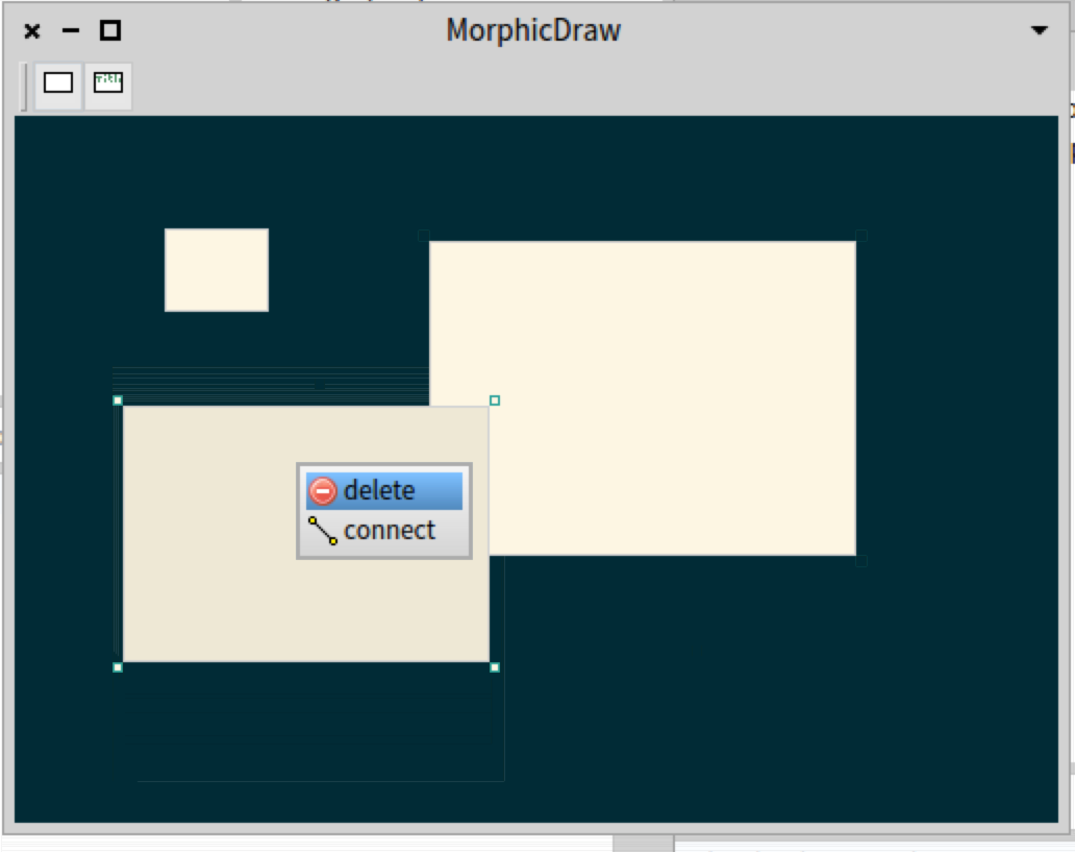
\includegraphics[width=200pt]{SimpleMorphicDrawWindow.pdf}
\caption{A first iteration of the main window of MorphicDraw}
\label{1stIteration}
\end{center}
\end{figure}
The first iteration (Figure \ref{1stIteration})  shows an application window 
with a toolbar and a drawing area. In the drawing area there are 
three graphical shapes, one of which is selected. A context menu
for the selected shape shows options to delete it and to connect it.


\section{Shapes and PasteUpMorph}

\section{Toolbar}
\section{Connecting}



\section{Selection and resizing}



\end{document}  